\chapter{Introduction}



The concept of sensory feedback is at the core of the study of cybernetics agents targeting autonomy. To realize
actions, an agent needs a representation of the current state of the world, which is inferred from its past sensors measurements. Current actions may 
then affect this state, which is reflected in a change of its sensors output. This creates a feedback loop, that, if designed well, leads to a stable, 
auto-regulated system.

For most robotics applications, the complexity of building a proper feedback behavior comes both from the difficulty
to capture a proper representation of the robot world and the diversity of possible control reactions. 
The world representation is built by an estimator that fuses several sources of information. 
The challenge is then to choose the set of appropriate sensors for each application and to design an efficient estimation algorithm to fuse them.
Let us first discuss how this feedback loop has evolved while robotics was growing mature.

% We will first compare the nature of perception needs for a few robotics applications, then give a biological example, and finish by motivating the use of 
% modular tightly-coupled estimators in the context of legged-robotics.



\section{From factory automation to dancing robots}


\begin{figure}[h]
    \centering
    \begin{subfigure}{0.3\textwidth}
        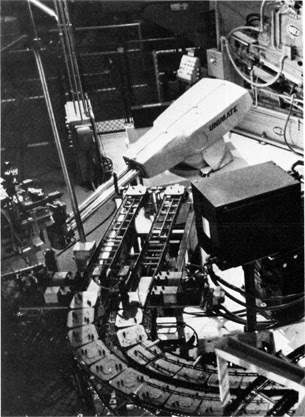
\includegraphics[width=\textwidth]{figures/1961unimate.jpg}
        \caption{}
        \label{fig:unimate}
    \end{subfigure}%
    \hspace{0.5cm}
    \begin{subfigure}{0.5\textwidth}
        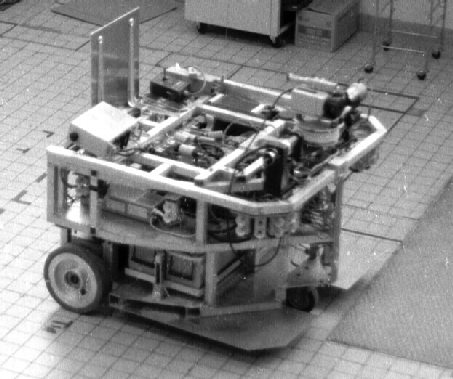
\includegraphics[width=\textwidth]{figures/hilare.png}
        \caption{}
        \label{fig:hilare}
    \end{subfigure}%

    \begin{subfigure}{0.49\textwidth}
        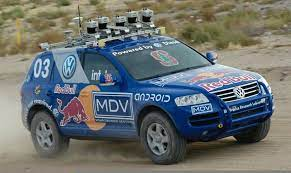
\includegraphics[width=\textwidth]{figures/darpa_car_stanford.jpeg}
        \caption{}
        \label{fig:darpa_stanford}
    \end{subfigure}%
    \hspace{0.5cm}
    \begin{subfigure}{0.44\textwidth}
        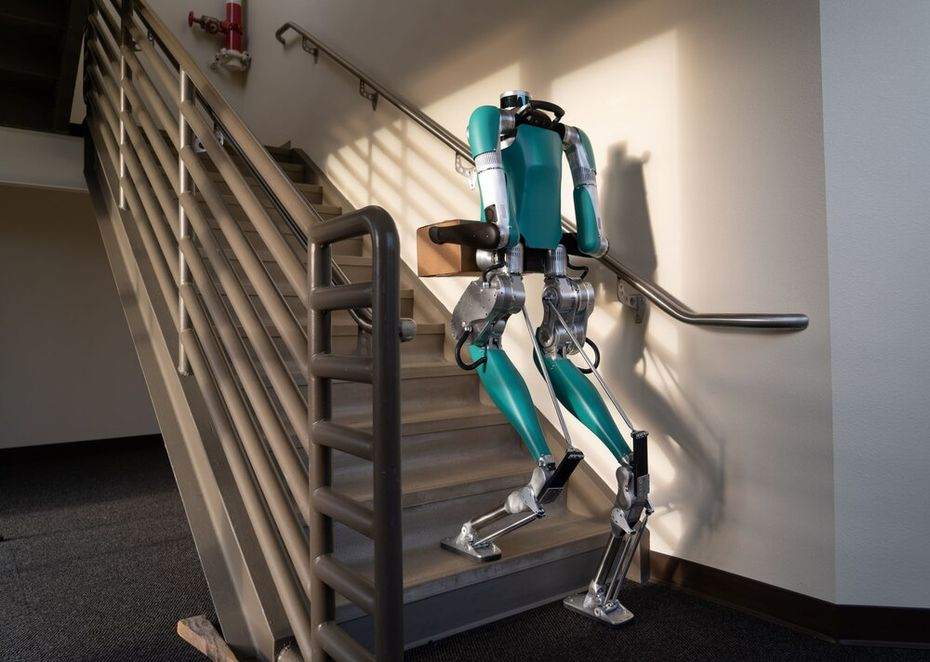
\includegraphics[width=\textwidth]{figures/digit.jpg}
        \caption{}
        \label{fig:digit}
    \end{subfigure}%
    \caption{Evolution of robotics platforms from factory manipulators to humanoid robots. (\subref{fig:unimate}) Unimate factory manipulator, 
    (\subref{fig:hilare}): Hilare mobile robotics research platform developed at LAAS-CNRS, (\subref{fig:darpa_stanford}): Stanford autonomous car winner of the 2005 grand challenge DARPA, 
    (\subref{fig:digit}): Digit (Agility Robotics) commercial humanoid robot.}

\end{figure}

Within the field of robotics, the implementation of the feedback loop has seen dramatic changes over the years, propelled by the changing nature 
of the mechatronic systems, in particular in the actuation and sensor array, the applications at play, and the mathematical formulations
used to model the systems. The progression of the perception side of the loop, extracting meaningful information from sensor data, can be divided into a few
steps that accompany the evolution of robotics, from fixed manipulators to agile legged robots. 

The first major robotic use was in the industrial space: 
starting in the early 60's \footnote{The Unimate manipulator was adopted by General Motors to displace hot die casting pieces to cooling tanks or assembly lines, first tests starting in 1961.}, 
arm manipulators have been progressively integrated into many assembly lines, especially in the automotive industry. 
This application requires the performance of highly precise, repetitive tasks, which are predefined by specialized human operators.
These highly rigid robots are controlled in position and fixed to the ground, which usually limits the perception needs to the relative angles between their different parts.

On the other end of the spectrum, researchers started to equip wheeled mobile platforms in controlled laboratory environments with exteroceptive sensors 
\cite{Nilsson1984ShakeyTR, chatila1985position} to apply planning algorithms, using mainly range sensors to control the presence of obstacles, along with wheel odometry \footnote{Odometry is, in the large sense, information 
about the relative motion of a robot obtained the integration of a motion sensor (wheel encoder, IMU, Doppler Velocity Logs, etc.)}
to detect relative displacement. 
Research on mobile robotics moved to outdoors applications, using motorized vehicles as research platforms. The 2005 DARPA grand challenge
offered one of the first large scale proof of concept of autonomous cars, where a few teams managed to safely drive 150 miles paths in desert-environments 
\cite{thrun2006stanley} (see \figRef{fig:darpa_stanford}), while the 2007 DARPA Urban challenge concentrated on urban road environments \cite{urmson2008autonomous}. In both cases, cars were 
equipped with GPS, IMU's, cameras, and a metric map of the path. Most teams relied heavily on global positioning, exteroceptive sensors being used for 
minor checks and corrections \cite{hillel2014recent}. Nowadays, the most successful autonomous car systems 
% (such as Tesla \footnote{See A. Karpathy \href{https://www.youtube.com/watch?v=g6bOwQdCJrc}{presentation} of Tesla's vision stack} and comma.ai \cite{comma2020openpilot}) 
seem to tend toward exclusive use of vision for local navigation (lane following, lane changing, overtaking, etc.) \footnote{As Andrej Karpathy puts it, “Lidar is really a shortcut”}. 

% Mature systems now exhibit almost human-level performance, though some hard corner cases,
% especially involving other humans behavior predictions, are still on the table.
% Though relying mostly on global positioning (fusing GPS and IMU \cite{hillel2014recent}), exteroceptive sensing 

In this landscape of autonomous systems, legged robots (humanoid or quadrupeds) are singular in many regards. 
First and foremost, they are inherently unstable dynamical systems that require continuous active control by applying forces at chosen locations of the environment. 
Therefore, they require an acute sense of balance, in which Inertial Measurement Units and contact detection play important roles. 
%which was primarily handled by Inertial Measurement Units in early applications ([CITE RAIBERT+HONDA]) 
Secondly, they are mobile platforms, whose primary function is to be able to navigate environments to perform tasks such as inspection or manipulation.
A perception of the environment is therefore required for any meaningful tasks to be undertaken, contrary to fixed manipulators.
Thirdly, they can in theory navigate cluttered, unstructured environments, which extends their operational capacities, compared to wheeled platforms.
This makes for challenging perceptual problems that require taking into account the many sensor modalities available.

In this thesis, we are interested in extending the perceptual capabilities of legged robots (humanoids and quadrupeds). This kind of robot requires both a high-rate (1kHz),
low latency estimates (<1ms) of its physical quantities to balance itself, like a precise direction of the gravity (< 0.01 radians for a full-size biped), 
and an accurate environment representation for safe navigation and interaction.
As we will explain in the next chapter, these tasks are oftentimes handled separately in the literature. We believe that it is possible to improve existing systems by a tight integration of the
many sensor modalities available on such a platform.

As a first justification of this point of view, let us consider first a biological example that will motivate the formulation of this approach.


\section{Biological equivalent, an example}

A digression through a biological example can give some intuitions to grasp the complexity of the problem. 
Let us investigate the example of a human lifting a box. Our vision might inform us about the general form of the object, 
its location in space with respect to us, some of its physical properties through our prior knowledge of the world. Our proprioception (kinesthetic sense) 
instinctively guide our arms toward the right path. Our sense of touch might infer the surface texture of the object,  its softness, making us 
adapt our grip. During this whole process, our vestibular system provides us with a sense of balance to counter gravity, while our ears 
make us aware of events external to our current enterprise.

All of this happens mostly at the subconscious level while our conscious mind focuses on high-level decisions.
The difficulty of mimicking these feats is therefore hard to grasp at first since we are most of the time oblivious to them.
However, if even one of these senses becomes deficient we are severely hindered in our daily enterprises. For instance, for people deprived
of proprioception, something as simple as grasping a glass while being seated is a tedious process, even if their sense of touch and vision works perfectly.


% Imitating these skills in robot system requires then to build models of available sensor modalities and to integrate them through the sensor
% fusion. 

% This can be achieved at several levels depending on the task to solve. In the legged robot community, one of the core tasks is locomotion.
% For this application, robust algorithms exist in the literature using a limited set of sensors, most often inertial and contact detection.
% On the other end of the blind robot approach, a broad field of research has been concentrated on building representations of the environment 
% using exteroceptive sensors such as cameras and LIDARs. This in turn enables planning algorithms to navigate the robot in its environment. 
% Many approaches decouple the two tasks, using layered perception systems. However, theoretically, a system able to tightly fuse all the 
% available modalities would benefit from a better consideration of the correlations between the different quantities to estimate. 
% Even though recent approaches have taken a step in this direction, such a system is still not widely used in legged robotics. 
% This thesis is a contribution to this goal. 




% For robots, perception of oneself and its environment is a major challenge on the road toward many real-world applications. 
% Tasks that are instinctive to us, like for instance manipulating an object, actually involve a complex 
% interactions between our many senses, our nervous and our muscular system.
% Though our sensory-motor skills have been developed by millions of years of evolution, and are refined throughout our childhood,
% the task of representing them in an abstracted algorithm to be implemented on a cybernetic system is a serious challenge. 


\section{How to implement artificial sensing for legged robots}

Legged robots are designed to evolve in human-designed environments to be able to replace us in some of our tedious or dangerous tasks. As such, they should be able to
display a sufficient level of dynamical intelligence and perception capabilities. 
In particular, the perception should be adapted to real-time control at the high frequencies usually found in legged-robot controllers (in the kilohertz range).
The estimated state should accurately reflect both the dynamics of the robot as well as its environment structure. Balance controllers in particular require a precise 
estimation of the gravity vector direction, as well centroidal quantities (center of mass, angular momentum, etc.).
In our opinion, this implies that the ideal perception system should encourage the multiplication of perception sources both in the number of sensors and their variety.
In addition, to maximize the accuracy of the estimator, any available correlations between variables and prior knowledge should in principle be taken into account. 
We also need to enable online calibration of the many sensor biases and fixed parameters. To achieve these goals, the development of \textit{tightly-coupled} estimators, 
which exploit as many data correlations as possible between the sensor measurements, should be undertaken.

Two main perception problems are typically considered onboard a legged robot. On the first hand, the sense of balance is replicated through high-frequency
local estimator fusing IMU and contact information to obtain the robot base velocity directed with respect to the gravity field. On the other hand,
exteroceptive sensors (camera, LIDARs) are used to localize the robot with respect to a large representation of its environment, ideally built on the flight.
This second layer is typically estimated at lower frequencies.

It is not exactly clear what is the optimal set of sensors that needs to be integrated on legged platforms (though Inertial Measurement Units, kinesthesis, and 
cameras or LIDARS are becoming more and more standard for industrial applications). This set may depend heavily on the type of application,
the size of the platform (LIDARS are too bulky for smaller quadrupeds), or the acceptable price range of the robot. Thus, it is important to allow
for a great \textit{modularity} in the design of estimators.
And even though modularity together with tight coupling may seem incompatible at first, we believe these two assets must be attained simultaneously.
We think that this can be done by different means. 
First, by using a factor graph formulation together with a modular front-end/back-end architecture, that naturally leads to a tightly-coupled, optimization based, Maximum-a-Posteriori estimation.
Second, by a flexible software architecture
that allows a general formulation of estimation problems (which is the endeavor of WOLF \cite{sola2021wolf}\footnote{The WOLF repository, documentation and examples can be 
found in \url{www.iri.upc.edu/wolf}}, that we have used and contributed to during the preparation of this thesis). Third, by endeavoring to generalize the mathematical formulations of the measurement models  as much as possible. 
 




\section{Thesis organization and contributions}

This thesis aims at I contributing to the estimation of legged robots by taking into account information from
many sensors, of many types, and in a modular way. Tightly-coupled estimation, whose necessity will be recurrently corroborated in this thesis, maximizes the observability
of the system, as opposed to loosely-coupled methods. In particular, tightly-coupled methods makes it possible to estimate the biases and calibration parameters
on top of states variables. The Maximum-a-Posteriori approach, which is best described with the Factor Graph framework, lends itself comfortably 
to tightly-coupled approaches. I shall seek to demonstrate it by formulating several measurement models, in particular generalizing some existing approaches to other sensor modalities
in the first part of this thesis. In the second part,
I will then display the operational capacity of the system on several proofs of concepts, building blocks for a future whole-body estimator, providing both gravity aware
estimation for balance control, and world reconstruction for navigation. Those intermediate systems will enable to experimentally qualify the performances, 
and feasability of the method.

This thesis is organized in two parts:

\bigskip
\textbf{Chapter 2} presents a literature overview of state estimation legged robots, that we will use to position our objectives.

\bigskip
\textbf{Chapter 3} serves as a general introduction to Factor Graph optimization using the Maximum-A-Posteriori. We emphasize the special treatment of variables 
belonging to manifolds and give a brief introduction to Lie theory, which is used extensively in \mbox{Chapter 6}.

\bigskip
\textbf{Chapter 4} describes two different measurement models used in the object-level visual-inertial systems that we built. 

\bigskip
\textbf{Chapter 5} presents the use of robot kinematics to obtain leg-odometry measurements. 

\bigskip
\textbf{Chapter 6} introduces a generalization of the IMU pre-integration theory. Examples of the classic on-manifold pre-integration are recalled and 
then extended to a compact Lie group formulation. 

\bigskip
The chapters of the second part present three different applications where we fuse several of the sensing modalities described so far.
Regarding their practical implementation, we contributed to different parts of the WOLF state estimation framework \cite{sola2021wolf} which was 
submitted to RAL journal this year. We present these applications in the chronological order of their development, reflecting the opinions that
we had at those respective times.

\bigskip
\textbf{Chapter 7} presents the first application, which is a visual-inertial object-level SLAM system based on fiducial markers. This chapter describes
results presented in Humanoids 2019 conference paper \cite{fourmy2019absolute}.

\bigskip
In \textbf{Chapter 8} we propose a whole-body (base and centroidal states) estimator based on the fusion of IMU, kinematics, and force-torque sensors. This
work was presented at ICRA 2021 conference \cite{fourmy2021contact}.

\bigskip
In \textbf{Chapter 9}, a visual-inertial SLAM system using deep-learning-based object pose estimation is presented. This work will be submitted to IROS 2022 conference \cite{debeunne2021cosyslam}.

\bigskip
In \textbf{Chapter 10}, we will present the conclusions and perspectives of this work.



